\documentclass[notes,blackandwhite,mathsans,usenames,dvipsnames]{beamer}

\usepackage{amsmath}
\usepackage{amssymb}
\usepackage{graphicx}
\usepackage{fancybox}
\usepackage{booktabs}
\usepackage{multirow,pxfonts}
\usepackage{cmbright}
\usepackage{xcolor}
\usepackage{color}
\usepackage{enumitem}
\usepackage{animate}
\usepackage{changepage}

\usepackage[T1]{fontenc}
\fontencoding{T1}  
\usepackage[utf8]{inputenc}


\usefonttheme{default}
\setbeamercovered{invisible}
\beamertemplatenavigationsymbolsempty

\makeatletter
\setbeamertemplate{footline}
{
  \leavevmode
  \hbox{
  \begin{beamercolorbox}[wd=0.97\paperwidth,ht=2.25ex,dp=2ex,right]{}
{\color{mcxs2} \insertframenumber{} / \inserttotalframenumber}
  \end{beamercolorbox}}%
}




\definecolor{mcxs1}{HTML}{05386B}
\definecolor{mcxs2}{HTML}{379683}
\definecolor{mcxs3}{HTML}{5CDB95}
\definecolor{mcxs4}{HTML}{8EE4AF}
\definecolor{mcxs5}{HTML}{EDF5E1}
\setbeamercolor{frametitle}{fg=mcxs2}
\AtBeginDocument{\color{mcxs1}}

\setbeamercolor{itemize item}{fg=mcxs1}
\setbeamercolor{itemize subitem}{fg=mcxs2}
\setbeamercolor{enumerate item}{fg=mcxs1}
\setbeamercolor{description item}{fg=mcxs1}

\setbeamertemplate{itemize item}[triangle]
\setbeamertemplate{itemize subitem}[circle]



\begin{document}
%\fontfamily{pag}\selectfont
%\setbeamerfont{title}{family=\fontfamily{pag}\selectfont}
%\setbeamerfont{frametitle}{family=\fontfamily{pag}\selectfont}
%\setbeamerfont{framesubtitle}{family=\fontfamily{pag}\selectfont}






{\setbeamercolor{background canvas}{bg=mcxs1}
\begin{frame}

\vspace{1cm}
\begin{tabular}{rl}
&\textbf{\LARGE\color{mcxs2} Macroeconometrics}\\[8ex]
\textbf{\Large\color{purple}Lecture 9}&\textbf{\Large\color{mcxs2}Forecasting with Bayesian VARs}\\[19ex]
&\textbf{\color{purple}Tomasz Wo\'zniak}\\[1ex]
&{\small\color{mcxs3} Department of Economics}\\
&{\small\color{mcxs3}University of Melbourne}
\end{tabular}

\end{frame}
}



{\setbeamercolor{background canvas}{bg=mcxs1}
\begin{frame}

\vspace{1cm}\textbf{\color{mcxs3}Predictive density: frequentist approach}

\bigskip\textbf{\color{mcxs2}Predictive density: Bayesian approach}

\bigskip\textbf{\color{mcxs3}Forecasting Australian real output and inflation}

\small
\vspace{1cm}{\color{mcxs2}Useful reading:} \\ \small
\smallskip{\color{mcxs4}Karlsson (2013) Forecasting with Bayesian Vector Autoregression, Handbook of Economic Forecasting}

\bigskip\small{\color{mcxs2}Materials:}\\ \footnotesize
{\color{mcxs4}An R file} {\color{mcxs3}\texttt{L9 mcxs.R}} {\color{mcxs4}for the reproduction the results}\\
{\color{mcxs4}A data file} {\color{mcxs3}\texttt{RGDP-RGDPDEF.csv}}
\end{frame}
}



{\setbeamercolor{background canvas}{bg=mcxs4}
\begin{frame}

\bigskip\textbf{\color{mcxs1}Objectives.}
\begin{itemize}[label=$\blacktriangleright$]
\item {\color{mcxs1}To introduce a full statistical characterisation of future unknown values of interest}
\item {\color{mcxs1}To present multivariate forecasting using Bayesian VARs}
\item {\color{mcxs1}To understand the difference between frequentist and Bayesian density forecasting}
\end{itemize}

\bigskip\textbf{\color{mcxs2}Learning outcomes.}
\begin{itemize}[label=$\blacktriangleright$]
\item {\color{mcxs2}Deriving the joint density of forecasted values}
\item {\color{mcxs2}Working on advanced transformation of normal distributions}
\item {\color{mcxs2}Reporting useful characteristics of the predictive densities}
\end{itemize}

\end{frame}
}



{\setbeamercolor{background canvas}{bg=mcxs4}
\begin{frame}{The objective of economic forecasting}

... is to use the available data to provide a statistical characterisation of the unknown future values of quantities of interest.

\bigskip The full statistical characterisation of the unknown future values of random variables is given by their {\color{mcxs2}predictive density.}

\bigskip Simplified outcomes in a form of statistics summarising the predictive densities are usually used in decision-making processes.

\bigskip Summary statistics are also communicated to general audiences.

\end{frame}
}





{\setbeamercolor{background canvas}{bg=mcxs1}
\begin{frame}

\begin{adjustwidth}{-0.5cm}{0cm}
%\FlushLeft
\vspace{8.3cm}\Large
\textbf{{\color{mcxs3}Predictive density:} {\color{mcxs5}frequentist approach}}
\end{adjustwidth}

\end{frame}
}



\begin{frame}{Predictive density: frequentist approach}

\textbf{VAR($p$) model.}
\begin{align*}
y_t &= {\color{purple}\mu_0} + {\color{purple}A_1} y_{t-1} + \dots + {\color{purple}A_p} y_{t-p} + \epsilon_t\\
\epsilon_t|Y_{t-1} &\sim iid\mathcal{N}_N\left(\mathbf{0}_N,{\color{purple}\Sigma}\right)
\end{align*}

\bigskip\textbf{Matrix notation.}
\begin{align*} 
Y &= X{\color{purple}A} + E\\
E|X &\sim\mathcal{MN}_{T\times N}\left(\mathbf{0}_{T\times N},{\color{purple}\Sigma}, I_T\right)
\end{align*} 
\footnotesize
$$ 
\underset{\color{mcxs2}(K\times N)}{{\color{purple}A}}=\begin{bmatrix} {\color{purple}\mu_0}'\\ {\color{purple}A_1}'\\ \vdots \\ {\color{purple}A_p}' \end{bmatrix} \quad
\underset{\color{mcxs2}(T\times N)}{Y}= \begin{bmatrix}y_1' \\ y_2'\\ \vdots \\ y_T'\end{bmatrix} \quad
\underset{\color{mcxs2}(K\times1)}{x_t}=\begin{bmatrix} 1\\ y_{t-1}\\ \vdots \\ y_{t-p} \end{bmatrix}\quad
\underset{\color{mcxs2}(T\times K)}{X}= \begin{bmatrix}x_1' \\ x_2' \\ \vdots \\ x_{T}'\end{bmatrix} \quad
\underset{\color{mcxs2}(T\times N)}{E}= \begin{bmatrix}\epsilon_1' \\ \epsilon_2' \\ \vdots \\ \epsilon_{T}'\end{bmatrix}
$$

{\color{mcxs2}where} $K=1+pN$

\end{frame}




\begin{frame}{Predictive density: frequentist approach}

\textbf{Predictive density.}
\begin{align*}
y_{t+1} &= {\color{purple}\mu_0} + {\color{purple}A_1} y_{t} + \dots + {\color{purple}A_p} y_{t-p+1} + \epsilon_{t+1}\\
\epsilon_{t+1}|Y_{t} &\sim iid\mathcal{N}_N\left(\mathbf{0}_N,{\color{purple}\Sigma}\right)\\[1ex]
&\downarrow\\[1ex]
%y_{t+1}|Y_{t} &\sim\mathcal{N}_N\left({\color{purple}\mu_0} + {\color{purple}A_1} y_{t} + \dots + {\color{purple}A_p} y_{t-p+1},{\color{purple}\Sigma}\right)\\[2ex]
p(y_{t+1}|Y_{t},{\color{purple}A},{\color{purple}\Sigma}) &=\mathcal{N}_N\left({\color{purple}\mu_0} + {\color{purple}A_1} y_{t} + \dots + {\color{purple}A_p} y_{t-p+1},{\color{purple}\Sigma}\right)\\[6ex]
Y &= X{\color{purple}A} + E\\
E|X &\sim\mathcal{MN}_{T\times N}\left(\mathbf{0}_{T\times N},{\color{purple}\Sigma}, I_T\right)\\[1ex]
&\downarrow\\[1ex]
%Y|X &\sim\mathcal{MN}_{T\times N}\left(X{\color{purple}A},{\color{purple}\Sigma}, I_T\right)\\[2ex]
p(Y|X,{\color{purple}A},{\color{purple}\Sigma}) &=\mathcal{MN}_{T\times N}\left(X{\color{purple}A},{\color{purple}\Sigma}, I_T\right)
\end{align*} 

\end{frame}







\begin{frame}{Predictive density: 1-period ahead forecast}
\small
\textbf{Data generating process.}
\begin{align*}
y_{t+1} &= \mu_0 + A_1 y_{t} + \dots + A_p y_{t-p+1} + \epsilon_{t+1}
\end{align*} 

\smallskip\textbf{1-period ahead forecast.}
\begin{align*}
\mathbb{E}[y_{t+1}|Y_t] &= \mu_0 + A_1 \mathbb{E}[y_{t}|Y_t] + \dots + A_p \mathbb{E}[y_{t-p+1}|Y_t] + \mathbb{E}[\epsilon_{t+1}|Y_t]\\
y_{t+1|t} &= \mu_0 + A_1 y_{t} + \dots + A_p y_{t-p+1}
\end{align*} 

\smallskip\textbf{1-period ahead forecast error.}
\begin{align*}
\mathbf{e}_{t+1|t} &= y_{t+1} - y_{t+1|t} = \epsilon_{t+1}
\end{align*} 

\smallskip\textbf{1-period ahead forecast error variance.}
\begin{align*}
\mathbb{V}\text{ar}[\mathbf{e}_{t+1|t}] &= \mathbb{E}\left[\mathbb{E}_t[\epsilon_{t+1}\epsilon_{t+1}']\right] = \Sigma 
\end{align*} 

\end{frame}



\begin{frame}{Predictive density: 2-period ahead forecast}
\small
\textbf{Data generating process.}
\begin{align*}
y_{t+2} &= \mu_0 + A_1 y_{t+1} + \dots + A_p y_{t-p+2} + \epsilon_{t+2}
\end{align*} 

\smallskip\textbf{2-period ahead forecast.}
\begin{align*}
\mathbb{E}[y_{t+2}|Y_t] &= \mu_0 + A_1 \mathbb{E}[y_{t+1}|Y_t] + \dots + A_p \mathbb{E}[y_{t-p+2}|Y_t] + \mathbb{E}[\epsilon_{t+2}|Y_t]\\
y_{t+2|t} &= \mu_0 + A_1 y_{t+1|t} + A_2 y_{t} + \dots + A_p y_{t-p+2}
\end{align*} 

\smallskip\textbf{2-period ahead forecast error.}
\begin{align*}
\mathbf{e}_{t+2|t} &= y_{t+2} - y_{t+2|t} = \epsilon_{t+2} + A_1(y_{t+1} - y_{t+1|t}) = \epsilon_{t+2} + A_1\epsilon_{t+1}
\end{align*} 

\smallskip\textbf{2-period ahead forecast error variance.}
\begin{align*}
\mathbb{V}\text{ar}[\mathbf{e}_{t+2|t}] &= \mathbb{E}[\mathbf{e}_{t+2|t}\mathbf{e}_{t+2|t}'] \\
&= \mathbb{E}[(\epsilon_{t+2} + A_1\epsilon_{t+1})(\epsilon_{t+2} + A_1\epsilon_{t+1})'] \\
&= \mathbb{E}\left[\mathbb{E}_{t+1}[\epsilon_{t+2}\epsilon_{t+2}']\right] + A_1\mathbb{E}\left[\mathbb{E}_t[\epsilon_{t+1}\epsilon_{t+1}']\right]A_1' \\
&= \Sigma + A_1\Sigma A_1' 
\end{align*} 

\end{frame}




\begin{frame}{Predictive density: frequentist approach}

\textbf{Covariance.}
\begin{align*}
\mathbb{C}\text{ov}[y_{t+1},y_{t+2}] &= \mathbb{E}\left[ (y_{t+1} - y_{t+1|t})(y_{t+2} - y_{t+2|t})' \right]\\
&= \mathbb{E}\left[ (\epsilon_{t+1})(\epsilon_{t+2} + A_1\epsilon_{t+1})' \right]\\
&= \mathbb{E}\left[ \mathbb{E}_t[\epsilon_{t+1}\epsilon_{t+1}']  \right]A_1' \\
&= \Sigma A_1'
\end{align*} 

\end{frame}





\begin{frame}{Predictive density: joint density}

\textbf{Joint predictive density of $y_{t+1}$ and $y_{t+2}$ given $Y_t, {\color{purple}A},{\color{purple}\Sigma}$.}
\begin{align*}
p(y_{t+1},y_{t+2}|Y_t, {\color{purple}A},{\color{purple}\Sigma}) &= p(y_{t+2}|y_{t+1},Y_t, {\color{purple}A},{\color{purple}\Sigma})p(y_{t+1}|Y_t, {\color{purple}A},{\color{purple}\Sigma})\\[2ex]
p(y_{t+2}|y_{t+1},Y_t, {\color{purple}A},{\color{purple}\Sigma}) &= \mathcal{N}_N\left(y_{t+2|t}, {\color{purple}\Sigma} + {\color{purple}A_1\Sigma A_1}'  \right)\\
p(y_{t+1}|Y_t, {\color{purple}A},{\color{purple}\Sigma}) &= \mathcal{N}_N\left(y_{t+1|t}, {\color{purple}\Sigma}\right)\\[1ex]
\downarrow&\\[1ex]
p\left(\begin{bmatrix}y_{t+1}\\ y_{t+2}\end{bmatrix}\Big|Y_t, {\color{purple}A},{\color{purple}\Sigma}\right) &= \mathcal{N}_{2N}\left(\begin{bmatrix} y_{t+1|t} \\ y_{t+2|t} \end{bmatrix}, \begin{bmatrix} {\color{purple}\Sigma} & {\color{purple}\Sigma A_1}' \\ {\color{purple}A_1\Sigma} & {\color{purple}\Sigma} + {\color{purple}A_1\Sigma A_1}' \end{bmatrix}\right)
\end{align*} 

\end{frame}



\begin{frame}{Predictive density: joint density}

\textbf{Joint predictive density of $y_{t+1}, y_{t+2}, \dots, y_{t+h}$ given $Y_t, {\color{purple}A},{\color{purple}\Sigma}$.}\footnotesize

$$
\mathcal{N}_{hN}\left(\begin{bmatrix} y_{t+1|t} \\ y_{t+2|t} \\ \vdots \\ y_{t+h|t} \end{bmatrix}, 
\begin{bmatrix} 
{\color{purple}\Sigma} & {\color{purple}\Sigma \Phi_1}' & \dots & {\color{purple}\Sigma \Phi_{h-1}}' \\ 
 & {\color{purple}\Sigma} + {\color{purple}\Phi_1\Sigma \Phi_1}' & \dots & {\color{purple}\Sigma\Phi_1}' + {\color{purple}\Phi_1\Sigma\Phi_2}' + \dots +{\color{purple}\Phi_{h-1}\Sigma\Phi_h}' \\
 &  & \ddots & \vdots\\
 &&& {\color{purple}\Sigma} + {\color{purple}\Phi_1\Sigma\Phi_1}' +  \dots + {\color{purple}\Phi_h\Sigma\Phi_h}'
 \end{bmatrix}\right)
$$

\normalsize
\bigskip\begin{description}
\item[${\color{purple}\Phi_i} = J{\color{purple}\mathbf{A}}^iJ'$] {\color{mcxs2}-- parameters of VMA($\infty$) representation of VAR($p$)}
\item[${\color{purple}\mathbf{A}}$] {\color{mcxs2}-- parameter matrix of VAR($1$) representation of VAR($p$)}

\bigskip\item[Elements below the main diagonal] {\color{mcxs2} of the covariance matrix are equal to the transpose of the corresponding elements above the main diagonal}
\end{description}

\end{frame}



\begin{frame}{Predictive density: frequentist approach}

\textbf{Predictive density using parameter estimates $\hat{A}, \hat\Sigma$.}

\begin{align*}
p\left(\begin{bmatrix}y_{t+1}\\ y_{t+2}\end{bmatrix}\Big|Y_t, {\color{purple}A},{\color{purple}\Sigma}\right)\Bigg|_{\begin{array}{c}{\color{purple}A}=\hat{A}\\ {\color{purple}\Sigma}=\hat\Sigma\end{array}} &= \mathcal{N}_{2N}\left(\begin{bmatrix} \hat{y}_{t+1|t} \\ \hat{y}_{t+2|t} \end{bmatrix}, \begin{bmatrix} \hat\Sigma & \hat\Sigma \hat{A}_1' \\ \hat{A}_1\hat\Sigma & \hat\Sigma + \hat{A}_1\hat\Sigma \hat{A}_1' \end{bmatrix}\right)
\end{align*} 

\begin{description}
\item[Predictive density]{\color{mcxs2} is evaluated by plugging in the estimates in the place of the parameters}
\item[Estimates of parameters]{\color{mcxs2}in forecasting applications are treated as not random}
\item[Estimation uncertainty]{\color{mcxs2}is ignored in forecasting applications}
\item[Forecast error variances]{\color{mcxs2}are underestimated}
\item[Predictive densities]{\color{mcxs2}might be inaccurate}
\item[Solution:]{\color{purple}Bayesian forecasting}
\end{description}

\end{frame}







\begin{frame}{Predictive density: frequentist approach}

\textbf{1-period ahead predictive density.}
\begin{align*}
p(y_{t+1}|x_{t+1},{\color{purple}A},{\color{purple}\Sigma}) &=\mathcal{N}_N\left(x_{t+1}'{\color{purple}A},{\color{purple}\Sigma}\right)\\[2ex]
p\left(y_{t+1}\Big|x_{t+1}, {\color{purple}A},{\color{purple}\Sigma}\right) &= \mathcal{MN}_{1\times N}\left( x_{t+1}'{\color{purple}A}, {\color{purple}\Sigma}, 1 \right)\\[5ex]
p(y_{t+1}|x_{t+1},Y,X,{\color{purple}A},{\color{purple}\Sigma})&\big|_{\begin{array}{c}{\color{purple}A}=\hat{A}\\{\color{purple}\Sigma}=\hat\Sigma\end{array}} =\mathcal{N}_N\left(x_{t+1}'\hat{A},\hat\Sigma\right)\\
p\left(y_{t+1}|x_{t+1},Y,X, {\color{purple}A},{\color{purple}\Sigma}\right)&\big|_{\begin{array}{c}{\color{purple}A}=\hat{A}\\{\color{purple}\Sigma}=\hat\Sigma\end{array}} = \mathcal{MN}_{1\times N}\left( x_{t+1}'\hat{A}, \hat\Sigma, 1 \right)
\end{align*} 

\end{frame}








{\setbeamercolor{background canvas}{bg=mcxs1}
\begin{frame}

\begin{adjustwidth}{-0.5cm}{0cm}
%\FlushLeft
\vspace{8.3cm}\Large
\textbf{{\color{mcxs2}Predictive density:} {\color{purple}Bayesian approach}}
\end{adjustwidth}

\end{frame}
}





\begin{frame}{Predictive density: Bayesian approach}

\textbf{Posterior density.}
\begin{align*} 
p\left( {\color{purple}A}, {\color{purple}\Sigma}|Y,X \right) &= p({\color{purple}A}|Y,X,{\color{purple}\Sigma})p\left( {\color{purple}\Sigma}|Y,X \right)\\[2ex]
p({\color{purple}A}|Y,X,{\color{purple}\Sigma}) &= \mathcal{MN}_{K\times N}\left( \overline{A},{\color{purple}\Sigma},\overline{V} \right)\\
p({\color{purple}\Sigma}|Y,X) &= \mathcal{IW}_N\left( \overline{S}, \overline{\nu} \right)\\[2ex]
\overline{V}&= \left( X'X + \underline{V}^{-1}\right)^{-1} \\
\overline{A}&= \overline{V}\left( X'Y + \underline{V}^{-1}\underline{A} \right)\\
\overline{\nu}&= T+\underline{\nu}\\
\overline{S}&= \underline{S}+Y'Y + \underline{A}'\underline{V}^{-1}\underline{A} - \overline{A}'\overline{V}^{-1}\overline{A}
\end{align*} 

\end{frame}



\begin{frame}{Predictive density: Bayesian approach}

\textbf{1-period ahead predictive density.}\small
\begin{align*} 
p(y_{t+1}|x_{t+1},Y,X) = \iint p(y_{t+1}|x_{t+1},Y,X,{\color{purple}A},{\color{purple}\Sigma})p\left( {\color{purple}A}, {\color{purple}\Sigma}|Y,X \right) d{\color{purple}A}d {\color{purple}\Sigma}
\end{align*} 

\normalsize\bigskip
\begin{description}
\item[Predictive density]{\color{mcxs2} is evaluated by integrating out the parameters from a joint distribution of the forecasted values $y_{t+1}$ and the parameters ${\color{purple}A}, {\color{purple}\Sigma}$}
\item[Integration]{\color{mcxs2} is performed with respect to posterior distribution}
\item[Parameters]{\color{mcxs2}are treated as unknown random variables}
\item[Estimation uncertainty]{\color{mcxs2}is incorporated into forecasting}
\item[Predictive densities]{\color{mcxs2}are accurate}
\end{description}

\end{frame}



\begin{frame}{Predictive density: Bayesian approach}

\textbf{1-period ahead predictive density.}\small
\begin{align*} 
p(y_{t+1}|x_{t+1},Y,X) &= \iint p(y_{t+1}|x_{t+1},Y,X,{\color{purple}A},{\color{purple}\Sigma})p\left( {\color{purple}A}, {\color{purple}\Sigma}|Y,X \right) d{\color{purple}A}d {\color{purple}\Sigma}\\[2ex]
p\left(y_{t+1}\Big|x_{t+1}Y,X, {\color{purple}A},{\color{purple}\Sigma}\right) &= \mathcal{MN}_{1\times N}\left( x_{t+1}'{\color{purple}A}, {\color{purple}\Sigma}, 1 \right)\\[2ex]
p\left( {\color{purple}A}, {\color{purple}\Sigma}|Y,X \right) &= p({\color{purple}A}|Y,X,{\color{purple}\Sigma})p\left( {\color{purple}\Sigma}|Y,X \right)\\
p({\color{purple}A}|Y,X,{\color{purple}\Sigma}) &= \mathcal{MN}_{K\times N}\left( \overline{A},{\color{purple}\Sigma},\overline{V} \right)\\
p({\color{purple}\Sigma}|Y,X) &= \mathcal{IW}_N\left( \overline{S}, \overline{\nu} \right)
\end{align*} 

\bigskip\normalsize{\color{mcxs2}Derive the solution step-by-step}
\begin{description}
\item[Step 1] Integrate out ${\color{purple}A}$
\item[Step 2] Integrate out ${\color{purple}\Sigma}$
\end{description}
\end{frame}









\begin{frame}{Useful distribution transformations}

\textbf{Linear combination of matrix-variate normal random variable.}
\begin{align*} 
{\color{purple}X}|\Sigma &\sim\mathcal{MN}_{K\times N}\left( M, \Sigma, V \right)\\
A{\color{purple}X}+a|\Sigma &\sim\mathcal{MN}_{L\times N}\left( AM+a, \Sigma, AVA' \right)\\
{\color{purple}X}B+b|\Sigma &\sim\mathcal{MN}_{K\times L}\left( MB+b, B\Sigma B', V \right)
\end{align*} 

\bigskip\textbf{Matrix-variate normal compound distribution.}
\begin{align*} 
{\color{purple}X}|{\color{purple}C},\Sigma &\sim\mathcal{MN}_{K\times N}\left( \overline{M}{\color{purple}C}, \Sigma, V \right)\\
{\color{purple}C}|\Sigma &\sim\mathcal{MN}_{L\times N}\left( \overline{C}, \Sigma, W \right)\\[2ex]
p({\color{purple}X}|\Sigma) &= \int p({\color{purple}X}|{\color{purple}C},\Sigma)p({\color{purple}C}|\Sigma)d{\color{purple}C}\\
&= \mathcal{MN}_{K\times N}\left( \overline{M}\overline{C}, \Sigma, V + \overline{M}W\overline{M}' \right)
\end{align*} 

\bigskip\footnotesize $\underset{\color{mcxs2}(K\times N)}{{\color{purple}X}}$, $\underset{\color{mcxs2}(K\times N)}{M}$, $\underset{\color{mcxs2}(K\times L)}{\overline{M}}$, $\underset{\color{mcxs2}(L\times N)}{C}$, $\underset{\color{mcxs2}(L\times N)}{\overline{C}}$, $\underset{\color{mcxs2}(L\times K)}{A}$, $\underset{\color{mcxs2}(L\times N)}{a}$, $\underset{\color{mcxs2}(N\times L)}{B}$, $\underset{\color{mcxs2}(K\times L)}{b}$, $\underset{\color{mcxs2}(N\times N)}{\Sigma}$, $\underset{\color{mcxs2}(K\times K)}{V}$, $\underset{\color{mcxs2}(L\times L)}{W}$

\end{frame}



\begin{frame}{Useful distributions: matric-variate t}

\textbf{Matric-variate t as a marginal distribution of $X$.}
\begin{align*} 
{\color{purple}X}|{\color{purple}\Sigma} &\sim\mathcal{MN}_{K\times N}\left( M, {\color{purple}\Sigma}, V \right)\\
{\color{purple}\Sigma} &\sim\mathcal{IW}_{N\times N}\left( S, \nu \right)\\
\downarrow&\\
p({\color{purple}X}) &=\int p({\color{purple}X}|{\color{purple}\Sigma}) p({\color{purple}\Sigma})d{\color{purple}\Sigma}\\
&=\mathcal{M}t_{K\times N}\left( M, V, S, \nu \right)
\end{align*} 
\textbf{Density function.}
\begin{align*} 
\mathcal{M}t_{K\times N}\left( M, V, S, \nu \right) &= {\color{mcxs2}c_{mt}^{-1}}\text{det}\left[S + ({\color{purple}X}-M)'V^{-1}({\color{purple}X}-M) \right]^{-\frac{\nu+K}{2}}\\
{\color{mcxs2}c_{mt}}&=\footnotesize {\color{mcxs2}\pi^{\frac{KN}{2}}\text{det}(V)^{\frac{N}{2}}\text{det}(S)^{-\frac{\nu}{2}}\left( \prod_{n=1}^{N} \frac{\Gamma\left(\frac{\nu+1-n}{2}\right)}{\Gamma\left(\frac{\nu+K+1-n}{2}\right)} \right)}
\end{align*} 

\end{frame}


\begin{frame}{Useful distributions: matrix-variate t}

$$ {\color{purple}X} \sim\mathcal{M}t_{K\times N}\left( M, V, S, \nu \right) $$

\bigskip\textbf{Moments.}
\begin{align*} 
\mathbb{E}[{\color{purple}X}]&= M &\text{\color{mcxs2} for }\nu&>N\\
\mathbb{V}\text{ar}[\text{vec}({\color{purple}X})]&= \frac{1}{\nu-N-1}S\otimes V &\text{\color{mcxs2} for }\nu&>N+1
\end{align*} 

\end{frame}




\begin{frame}{Predictive density: Bayesian approach}

\textbf{1-period ahead predictive density.}

\bigskip\textbf{Step 1: Integrate out ${\color{purple}A}$:}
\begin{align*} 
p(y_{t+1}|x_{t+1},Y,X,{\color{purple}\Sigma}) &= \int p(y_{t+1}|x_{t+1},Y,X,{\color{purple}A},{\color{purple}\Sigma})p({\color{purple}A}|Y,X,{\color{purple}\Sigma}) d{\color{purple}A}\\[2ex]
p\left(y_{t+1}\Big|x_{t+1}Y,X, {\color{purple}A},{\color{purple}\Sigma}\right) &= \mathcal{MN}_{1\times N}\left( x_{t+1}'{\color{purple}A}, {\color{purple}\Sigma}, 1 \right)\\
p({\color{purple}A}|Y,X,{\color{purple}\Sigma}) &= \mathcal{MN}_{K\times N}\left( \overline{A},{\color{purple}\Sigma},\overline{V} \right)\\
\downarrow&\\
p(y_{t+1}|x_{t+1},Y,X,{\color{purple}\Sigma}) &= \mathcal{MN}_{1\times N}\left( x_{t+1}'\overline{A}, {\color{purple}\Sigma}, 1 + x_{t+1}'\overline{V}x_{t+1} \right)
\end{align*} 

\end{frame}



\begin{frame}{Predictive density: Bayesian approach}

\textbf{1-period ahead predictive density.}

\bigskip\textbf{Step 2: Integrate out ${\color{purple}\Sigma}$:}
\begin{align*} 
p(y_{t+1}|x_{t+1},Y,X) &= \int p(y_{t+1}|x_{t+1},Y,X,{\color{purple}\Sigma})p({\color{purple}\Sigma}|Y,X) d{\color{purple}\Sigma}\\[2ex]
p(y_{t+1}|x_{t+1},Y,X,{\color{purple}\Sigma}) &= \mathcal{MN}_{1\times N}\left( x_{t+1}'\overline{A}, {\color{purple}\Sigma}, 1 + x_{t+1}'\overline{V}x_{t+1} \right)\\
p({\color{purple}\Sigma}|Y,X) &= \mathcal{IW}_N\left( \overline{S}, \overline{\nu} \right)\\
\downarrow&\\
p(y_{t+1}|x_{t+1},Y,X) &= \mathcal{M}t_{1\times N}\left( x_{t+1}'\overline{A}, 1 + x_{t+1}'\overline{V}x_{t+1}, \overline{S}, \overline{\nu} \right)
\end{align*} 

\end{frame}



\begin{frame}{Predictive density: Bayesian vs. frequentist approach}

\textbf{1-period ahead predictive density.}
\begin{align*} 
p(y_{t+1}|x_{t+1},Y,X) &= \mathcal{M}t_{1\times N}\left( x_{t+1}'\overline{A}, 1 + x_{t+1}'\overline{V}x_{t+1}, \overline{S}, \overline{\nu} \right)\\[1ex]
{\color{mcxs2}\mathbb{E}[y_{t+1}|x_{t+1},Y,X]} &= {\color{mcxs2}x_{t+1}'\overline{A}}\\
{\color{mcxs2}\mathbb{V}\text{ar}[y_{t+1}|x_{t+1},Y,X]} &= {\color{mcxs2}\frac{1+x_{t+1}'\overline{V}x_{t+1}}{\overline{\nu}-N-1}\overline{S}}\\[4ex]
p\left(y_{t+1}|x_{t+1},Y,X, {\color{purple}A},{\color{purple}\Sigma}\right)&\big|_{\begin{array}{c}{\color{purple}A}=\hat{A}\\{\color{purple}\Sigma}=\hat\Sigma\end{array}} = \mathcal{MN}_{1\times N}\left( x_{t+1}'\hat{A}, \hat\Sigma, 1 \right)\\
{\color{mcxs2}\mathbb{E}[y_{t+1}|x_{t+1},Y,X]} &= {\color{mcxs2}x_{t+1}'\hat{A}}\\
{\color{mcxs2}\mathbb{V}\text{ar}[y_{t+1}|x_{t+1},Y,X]} &= {\color{mcxs2}\hat\Sigma}
\end{align*} 

\end{frame}




\begin{frame}{Predictive density: Bayesian approach}

\textbf{Joint predictive density.}
\begin{align*}
p\left(Y_{t+h}\big|Y_t, {\color{purple}A},{\color{purple}\Sigma}\right)&= \mathcal{N}_{hN}\left(Y_{t+h|t}({\color{purple}A}), \mathbb{V}\text{ar}\left[Y_{t+h|t}\big| {\color{purple}A},{\color{purple}\Sigma}\right]\right)
\end{align*} 

\scriptsize\bigskip
$$ \underset{\color{mcxs2}(hN\times1)}{Y_{t+h}} = \begin{bmatrix}y_{t+1}\\ y_{t+2}\\ \vdots \\ y_{t+h} \end{bmatrix}\qquad \underset{\color{mcxs2}(hN\times1)}{Y_{t+h|t}}({\color{purple}A}) = \begin{bmatrix}y_{t+1|t}\\ y_{t+2|t}\\ \vdots \\ y_{t+h|t} \end{bmatrix} $$
$$\mathbb{V}\text{ar}\left[Y_{t+h|t}\big| {\color{purple}A},{\color{purple}\Sigma}\right] = \begin{bmatrix} 
{\color{purple}\Sigma} & {\color{purple}\Sigma \Phi_1}' & \dots & {\color{purple}\Sigma \Phi_{h-1}}' \\ 
 & {\color{purple}\Sigma} + {\color{purple}\Phi_1\Sigma \Phi_1}' & \dots & {\color{purple}\Sigma\Phi_1}' + {\color{purple}\Phi_1\Sigma\Phi_2}' + \dots +{\color{purple}\Phi_{h-1}\Sigma\Phi_h}' \\
 &  & \ddots & \vdots\\
 &&& {\color{purple}\Sigma} + {\color{purple}\Phi_1\Sigma\Phi_1}' +  \dots + {\color{purple}\Phi_h\Sigma\Phi_h}'
 \end{bmatrix} $$

\end{frame}





\begin{frame}{Predictive density: Bayesian approach}

\textbf{Joint predictive density.}

\begin{align*} 
p\left(Y_{t+h}\big|Y_t\right) = \int &p\left(Y_{t+h}\big|Y_t, {\color{purple}A},{\color{purple}\Sigma}\right)p\left( {\color{purple}A}, {\color{purple}\Sigma}|Y,X \right) d({\color{purple}A}, {\color{purple}\Sigma}) \\[2ex]
p\left(y_{t+h}\Big|Y,X, {\color{purple}A},{\color{purple}\Sigma}\right) &= \mathcal{N}_{hN}\left(Y_{t+h|t}({\color{purple}A}), \mathbb{V}\text{ar}\left[Y_{t+h|t}\big| {\color{purple}A},{\color{purple}\Sigma}\right]\right)\\
p\left( {\color{purple}A}, {\color{purple}\Sigma}|Y,X \right) &= \mathcal{NIW}_{K\times N}\left( \overline{A},\overline{V}, \overline{S}, \overline{\nu} \right)
\end{align*} 

\bigskip{\color{mcxs2}The analytical solution to the problem cannot be found.}\\
{\color{purple}Solution: use numerical integration.}
\end{frame}



\begin{frame}{Predictive density: Bayesian approach}

\textbf{Sampling the joint predictive density (Algorithm 1).}

\bigskip
\begin{description}
\item[Sample] {\color{mcxs2}draws from} $p({\color{purple}A}, {\color{purple}\Sigma}|Y,X)$ {\color{mcxs2}and} 
\item[Obtain] $\left\{ A^{(s)}, \Sigma^{(s)}\right\}_{s=1}^{S}$
\item[Sample] {\color{mcxs2}draws from} $\hat{p}\left(Y_{t+h}\big|Y_t\right)$ {\color{mcxs2}by:}
$$ Y_{t+h}^{(s)}\sim \mathcal{N}_{hN}\left(Y_{t+h|t}\left(A^{(s)}\right), \mathbb{V}\text{ar}\left[Y_{t+h|t}\big| A^{(s)},\Sigma^{(s)}\right]\right) $$
\item[Obtain] $\left\{ Y_{t+h}^{(s)}\right\}_{s=1}^{S}$
\item[Characterise] {\color{mcxs2}of the predictive density using} $\left\{ Y_{t+h}^{(s)}\right\}_{s=1}^{S}$
\end{description}

\end{frame}





{\setbeamercolor{background canvas}{bg=mcxs1}
\begin{frame}

\begin{adjustwidth}{-0.5cm}{0cm}
%\FlushLeft
\vspace{8.3cm}\Large
\textbf{{\color{mcxs2}Forecasting Australian} {\color{mcxs3}real output and prices}}
\end{adjustwidth}

\end{frame}
}


\begin{frame}{Australian real output and prices}

\centering
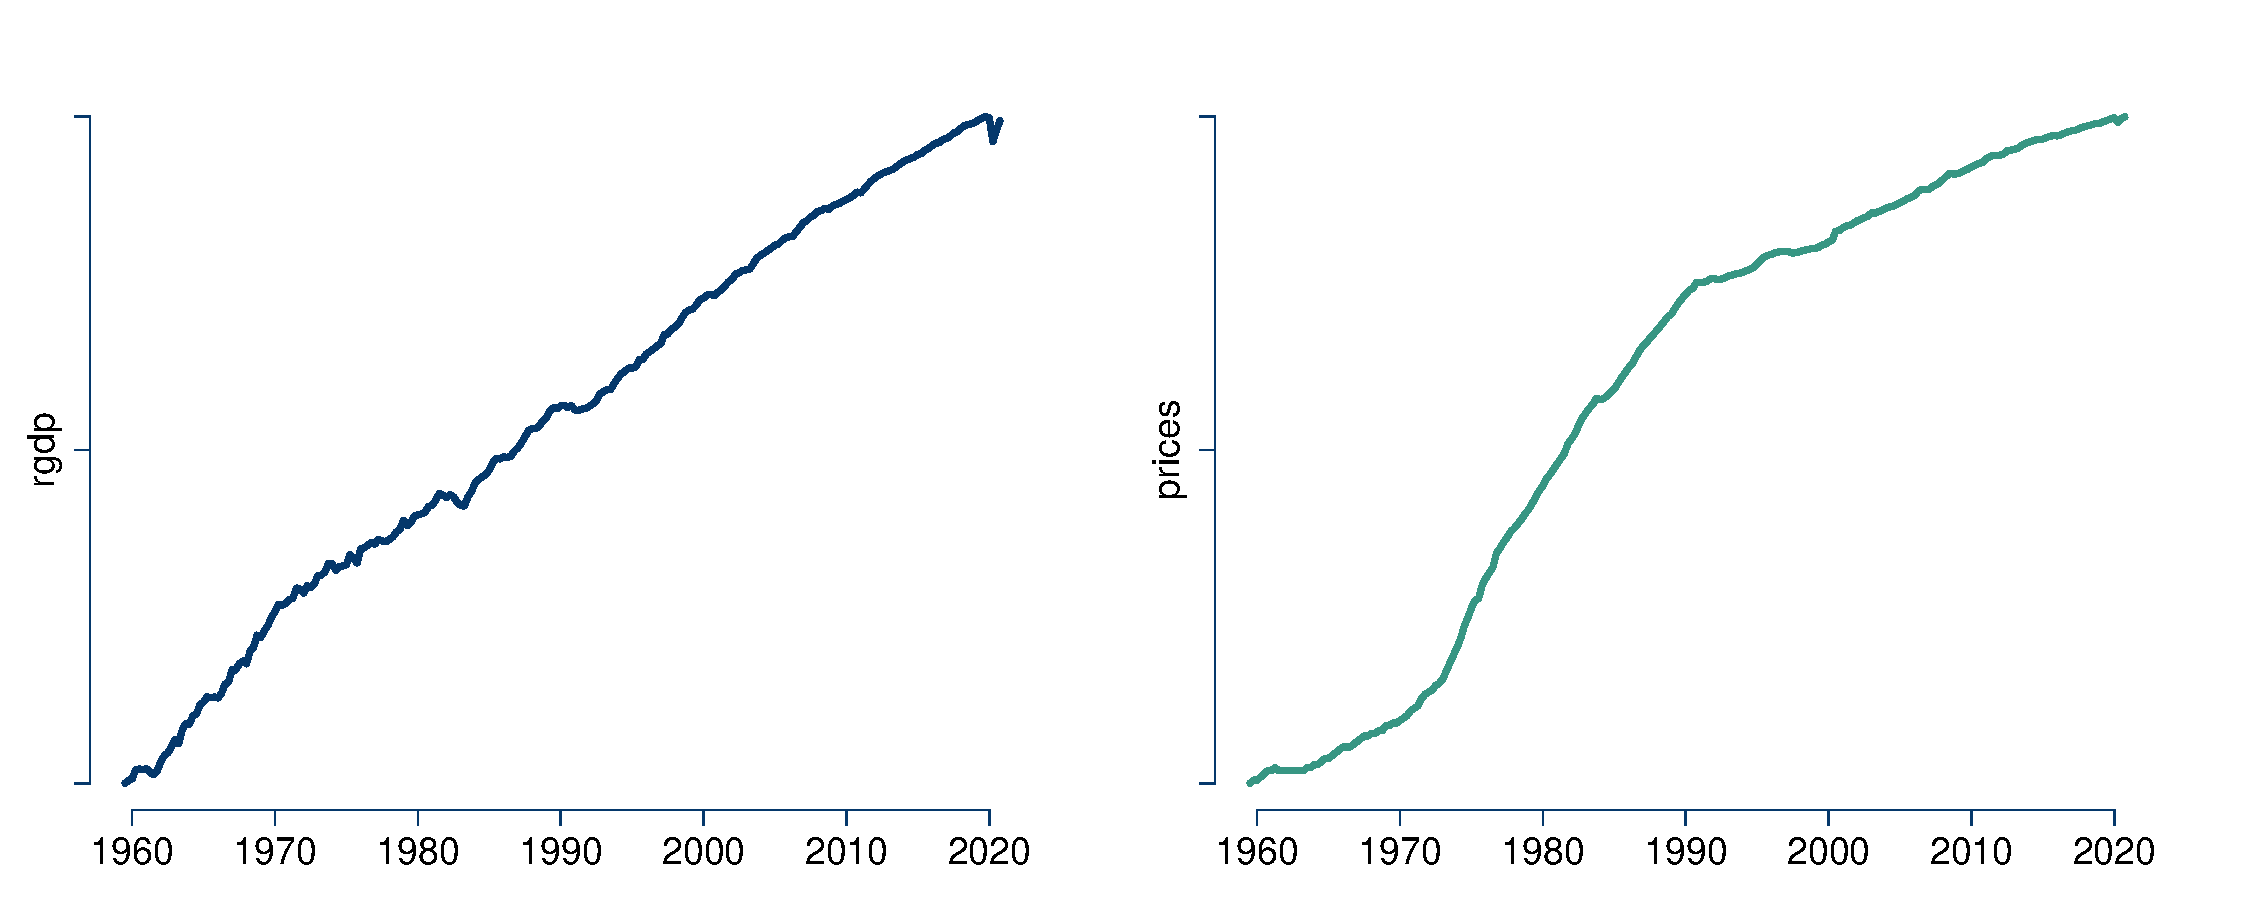
\includegraphics[scale=0.3]{data.pdf}

\bigskip{\color{mcxs2}Logarithms of real GDP and the CPI\\[1ex]
Sample period: 1959Q3 -- 2020Q4, $T$=246\\
Data source: Australian Macro Database: \href{http://ausmacrodata.org/}{ausmacrodata.org}
}
\end{frame}



\begin{frame}{Australian real output and prices}


\begin{adjustwidth}{-0.5cm}{0cm}
\centering
\textbf{Posterior estimates of the parameters of the VAR(4) model}

\smallskip\tiny
\begin{tabular}{ccccccccc}
  \toprule
\multicolumn{9}{c}{\normalsize${\color{purple}A}|Y,X$}\\[1ex]
$\mu_2$ & \multicolumn{2}{c}{$A_1$} & \multicolumn{2}{c}{$A_2$} & \multicolumn{2}{c}{$A_3$} & \multicolumn{2}{c}{$A_4$} \\ 
  \midrule
.010029 &  .999925 & -.000114 & -.000019 & -.000030 & -.000008 & -.000012 & -.000005 & -.000007\\[0ex]
[.00473] & [.00031] & [.00031] & [.00016] & [.00016] & [.00011] & [.00011] & [.00008] & [.00008] \\[1ex] 
 .015123 & -.000150 &  .999762 & -.000036 & -.000061 & -.000016 & -.000027 & -.000009 & -.000016 \\ [0ex]
[.00398] & [.00026] & [.00026] & [.00013] & [.00013] & [.00009] & [.00009] & [.00007] & [.00007] \\[1ex]
\midrule
& \multicolumn{2}{c}{\normalsize${\color{purple}\Sigma}|Y,X$}\\[1ex]
&  0.000253 & -0.000005 \\ 
& [0.00002] & [0.00001] \\ [1ex]
& -0.000005 &  0.000177 \\ 
& [0.00001] & [0.00002] \\ 
   \bottomrule
\end{tabular}
\end{adjustwidth}

\bigskip\small{\color{mcxs2}The table reports posterior means and [standard deviations] based on 50,000 draws from the posterior distribution.\\ Minnesota prior specified as in the slides is used. }

\end{frame}




\begin{frame}{Australian real output and prices forecasts}

\centering
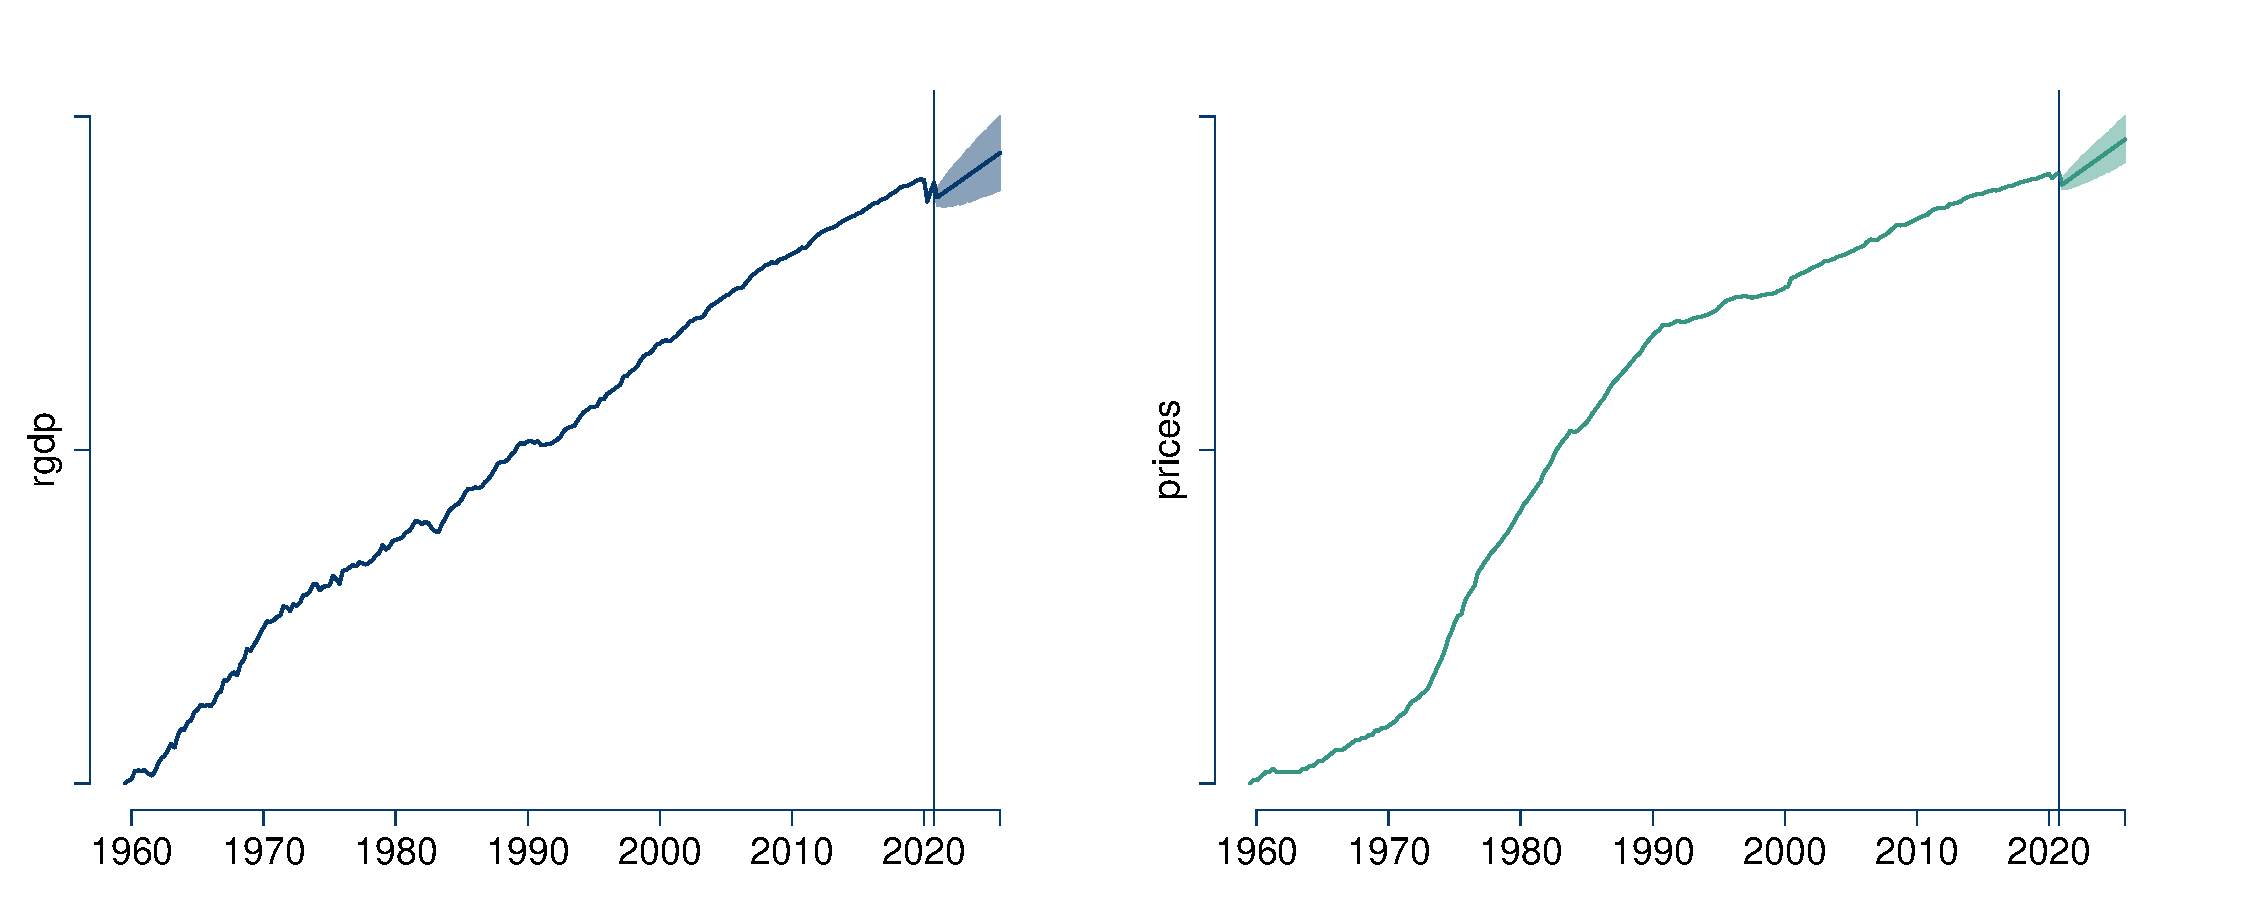
\includegraphics[scale=0.33, trim=2cm 0cm 0cm 0cm]{forecasts.pdf}

\bigskip{\color{mcxs2}Data and forecasts plot\\[1ex]
The forecasts are presented using predictive density means and 90\% highest density intervals 
}
\end{frame}





\begin{frame}{Joint predictive density 1-period ahead}

\centering
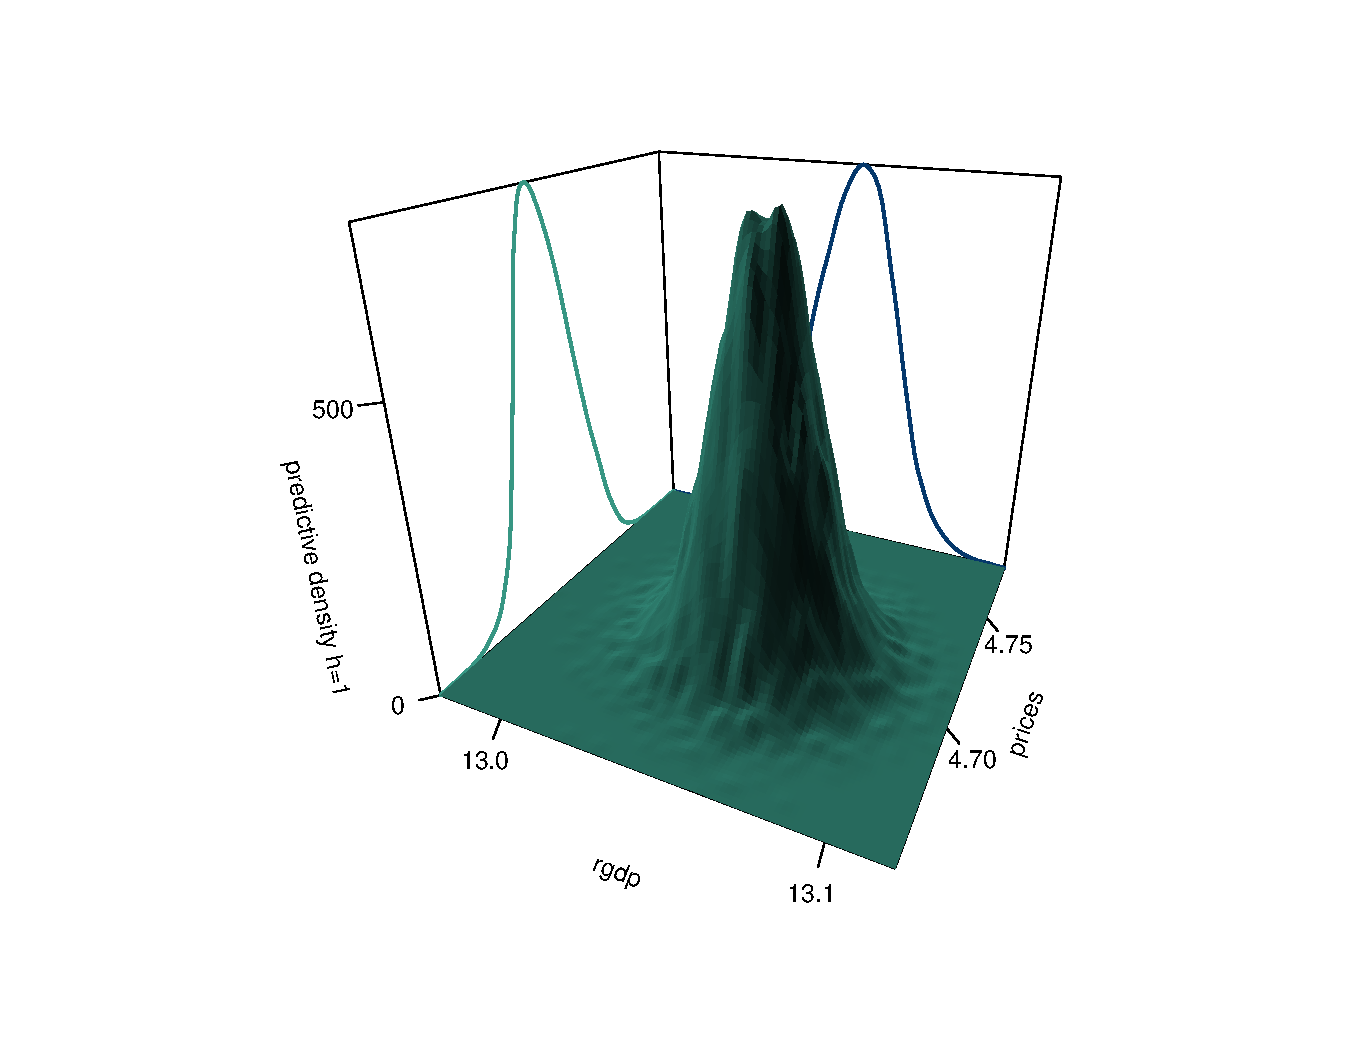
\includegraphics[scale=0.45, trim=0cm 2cm 0cm 0cm]{joint-predictive-1ph.pdf}

\footnotesize$\mathbb{C}\text{or}(rgdp_{t+1},p_{t+1}|Y_t)=-0.24$

\end{frame}



\begin{frame}{Joint predictive density 1 and 2 periods ahead}

\centering
\begin{tabular}{cc}
rgdp & {\color{mcxs2}prices}\\
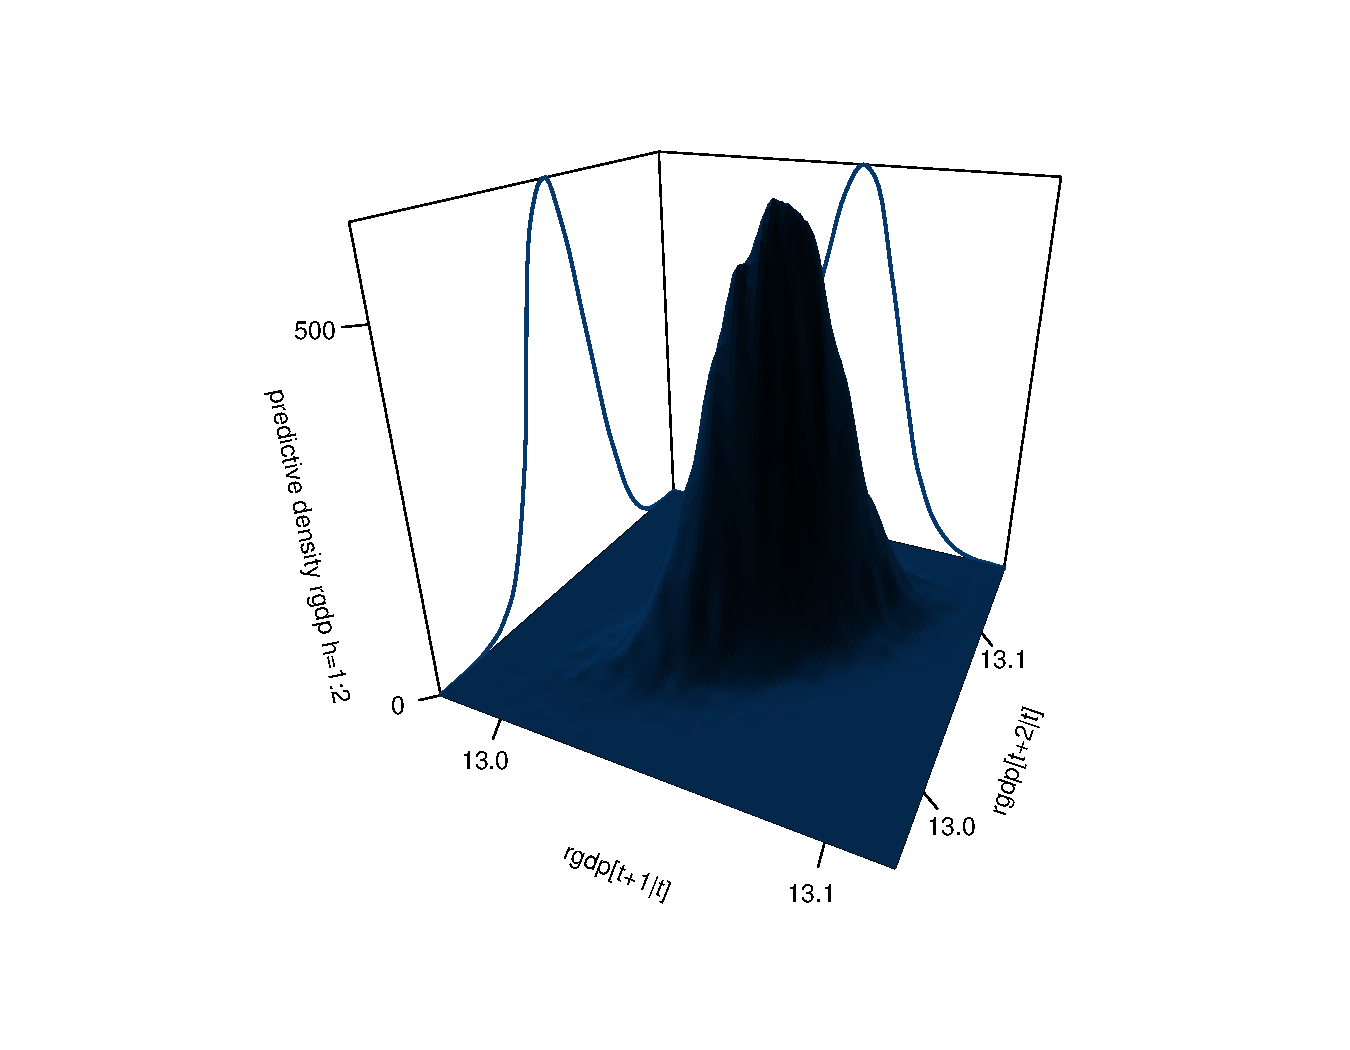
\includegraphics[scale=0.35, trim=4cm 2cm 4cm 2cm]{joint-predictive-rgdp-1and2ph.pdf} &
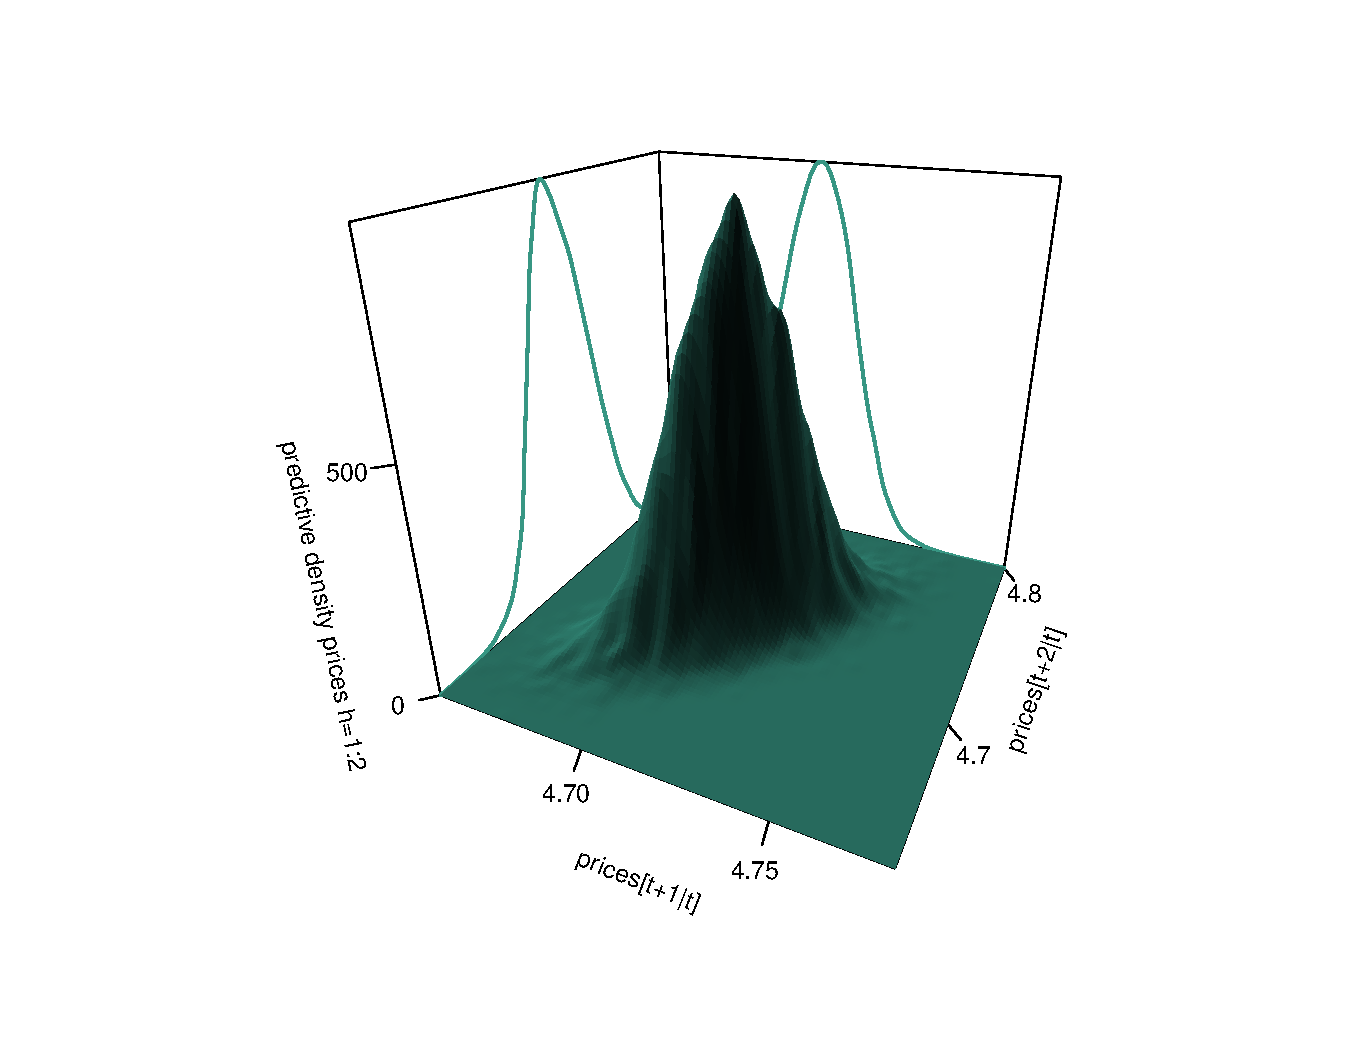
\includegraphics[scale=0.35, trim=4cm 2cm 4cm 2cm]{joint-predictive-prices-1and2ph.pdf}\\
\footnotesize$\mathbb{C}\text{or}(rgdp_{t+1},rgdp_{t+2}|Y_t)=0.71$ &
\footnotesize$\mathbb{C}\text{or}(p_{t+1},p_{t+2}|Y_t)=0.71$ 
\end{tabular}

\end{frame}



\begin{frame}{Predictive densities at all horizons}

\centering
\begin{tabular}{cc}
rgdp & {\color{mcxs2}prices}\\
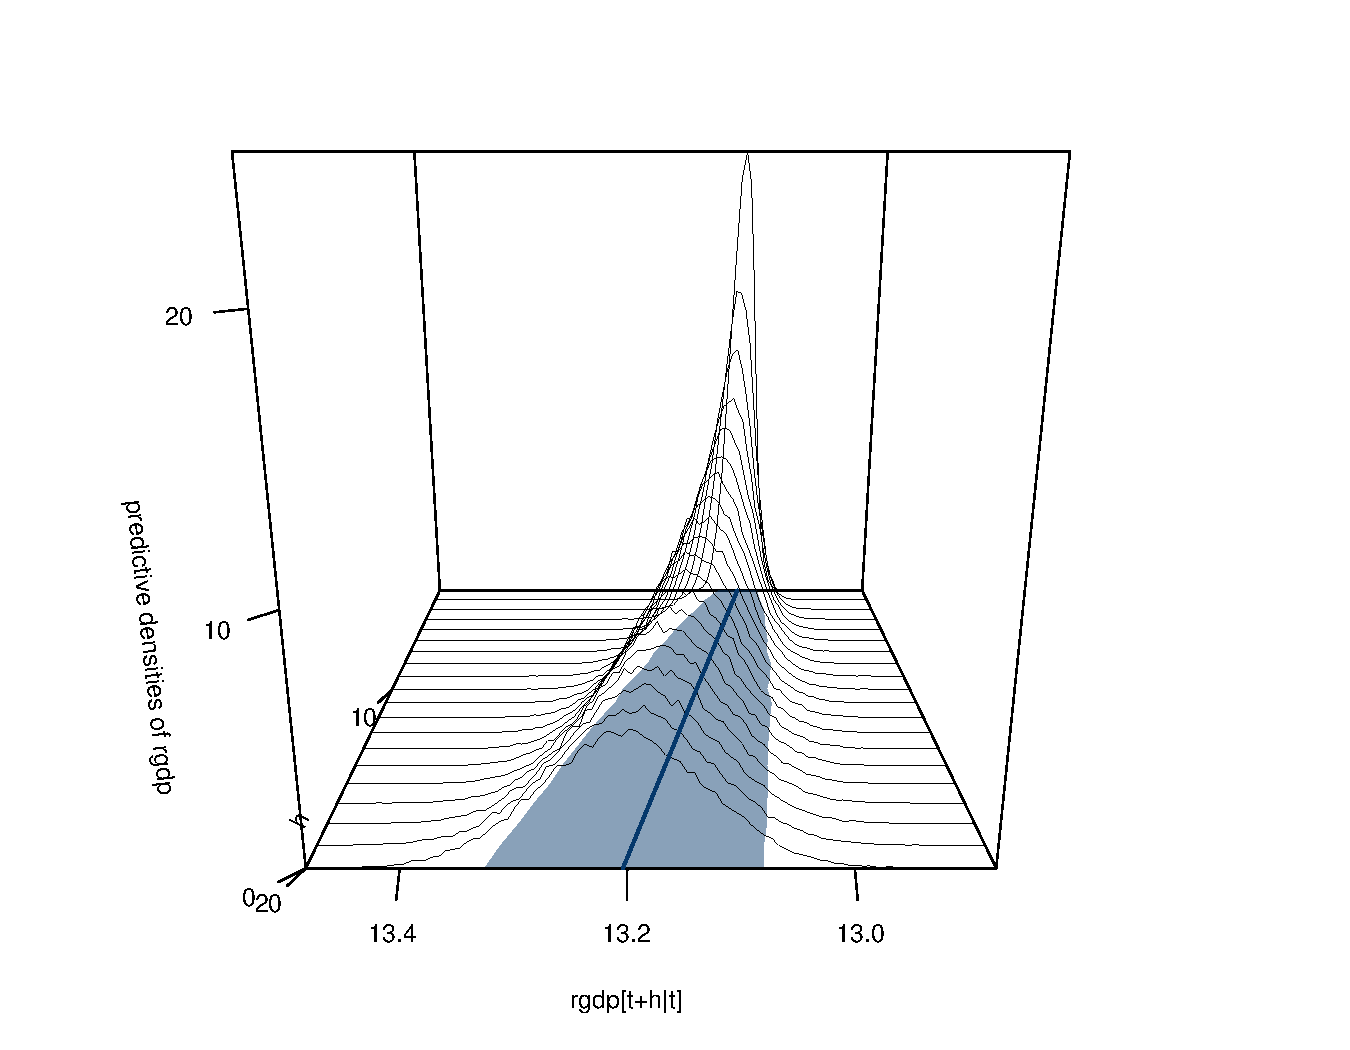
\includegraphics[scale=0.35, trim=4cm 2cm 4cm 2cm]{predictive-rgdp-horizons.pdf} &
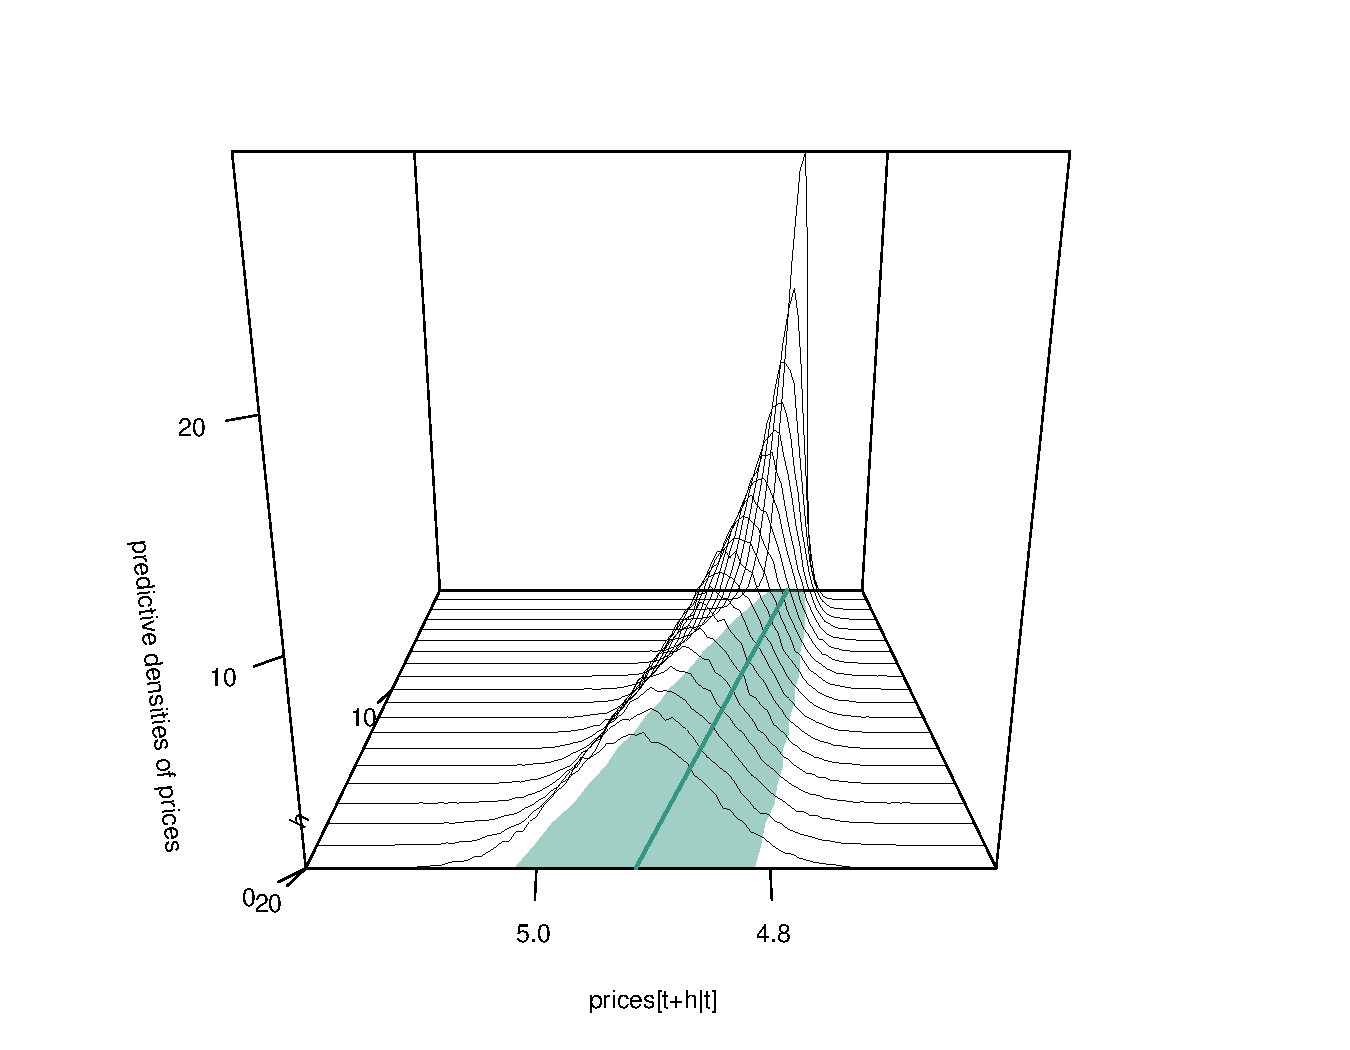
\includegraphics[scale=0.35, trim=4cm 2cm 4cm 2cm]{predictive-prices-horizons.pdf}
\end{tabular}

\end{frame}


{\setbeamercolor{background canvas}{bg=mcxs1}
\begin{frame}{\color{mcxs3}Forecasting with Bayesian VARs}

\begin{description}
\item[\color{mcxs3}Predictive densities] {\color{mcxs5}contain the full statistical characterisation of future unknown values of interest}

\bigskip\item[\color{mcxs3}Bayesian predictive densities] {\color{mcxs5}incorporate estimation uncertainty and differ with that respect from frequentist ones}

\bigskip\item[\color{mcxs3}Forecasts] {\color{mcxs5}inherit the properties of the stochastic process on which they are based}
\end{description}

\end{frame}
}




%\begin{frame}{Rao-Blackwellization}
%
%\textbf{Numerical integration to compute marginal densities.}
%
%\small{\color{mcxs2}Gelfand, Smith (1990, JASA), Sampling-Based Approaches to Calculating Marginal Densities}
%
%\normalsize\bigskip\textbf{The problem.}
%
%{\color{mcxs2}No analytical solution can be derived for}
%$$ p(Y) = \int p(Y,X)dX = \int p(Y|X)p(X)dX $$
%
%\bigskip\textbf{Solution.}
%\begin{description}
%\item[Sample] draws from $p(X)$ and obtain $\left\{ X^{(s)}\right\}_{s=1}^{S}$
%\item[Estimate] $\hat{p}(Y)$ by computing:
%$$ \hat{p}(Y) = \frac{1}{S}\sum_{s=1}^{S}p\left(Y|X^{(s)}\right) $$
%\end{description}
%
%\end{frame}
%
%
%
%\begin{frame}{Rao-Blackwellization for predictive density}
%
%\textbf{Numerical integration of joint predictive density.}
%
%\bigskip
%\begin{description}
%\item[Sample] draws from $p({\color{purple}A}, {\color{purple}\Sigma}|Y,X)$ and 
%\item[Obtain] $\left\{ A^{(s)}, \Sigma^{(s)}\right\}_{s=1}^{S}$
%\item[Estimate] $\hat{p}\left(Y_{t+h}\big|Y_t\right)$ by computing:
%$$ \hat{p}\left(Y_{t+h}\big|Y_t\right) = \frac{1}{S}\sum_{s=1}^{S}p\left(Y_{t+h}\big|Y_t, A^{(s)},\Sigma^{(s)}\right) $$
%\end{description}
%
%\bigskip{\color{mcxs2}To obtain smooth visualisation of the predictive densities at each forecasting horizon propose a representative grid of values for} $Y_{t+h}$ {\color{mcxs2}denoted by} $Y_{t+h}^{[1]}, \dots,Y_{t+h}^{[J]}$ {\color{mcxs2}and compute the predictive density estimate for each of the values from the grid} $\hat{p}\left(Y_{t+h}^{[j]}\big|Y_t\right)$.
%
%\end{frame}




\end{document} 